\begin{frame}{Teaching FEM basics}

\begin{columns}
\column{0.5\textwidth}
\begin{center}
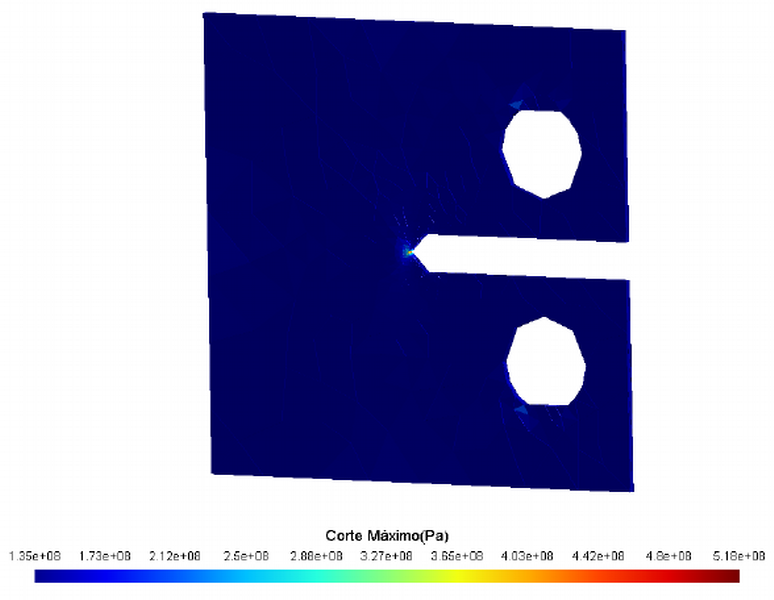
\includegraphics[height=0.5\textheight,width=\textwidth]{/home/mariano/CuadernoTrabajo/CV/SLI/03-Teaching/01.png}

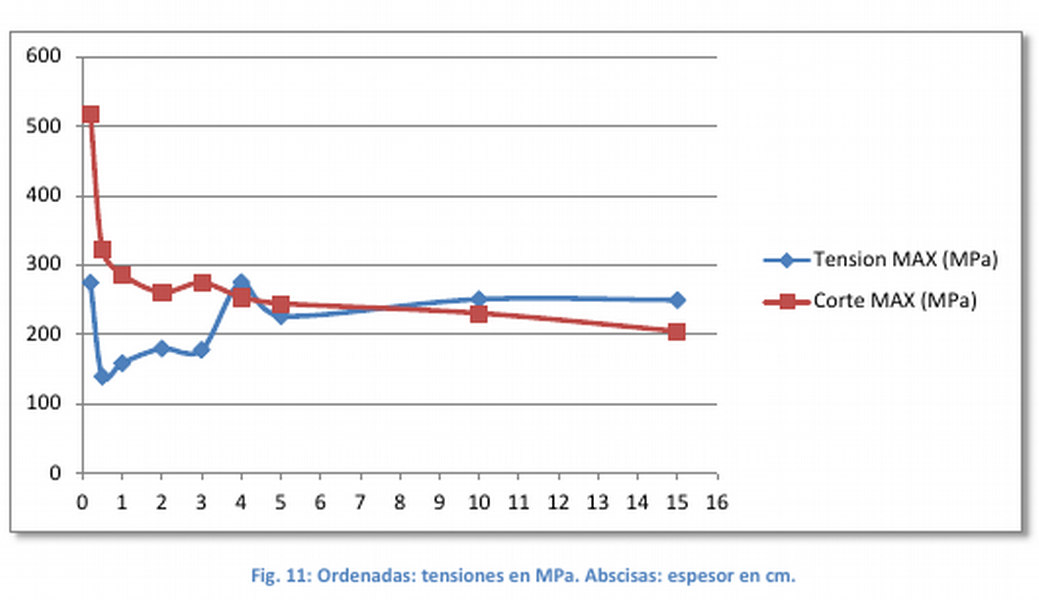
\includegraphics[height=0.3\textheight]{/home/mariano/CuadernoTrabajo/CV/SLI/03-Teaching/3.png}
\end{center}
\column{0.5\textwidth}
\begin{center}
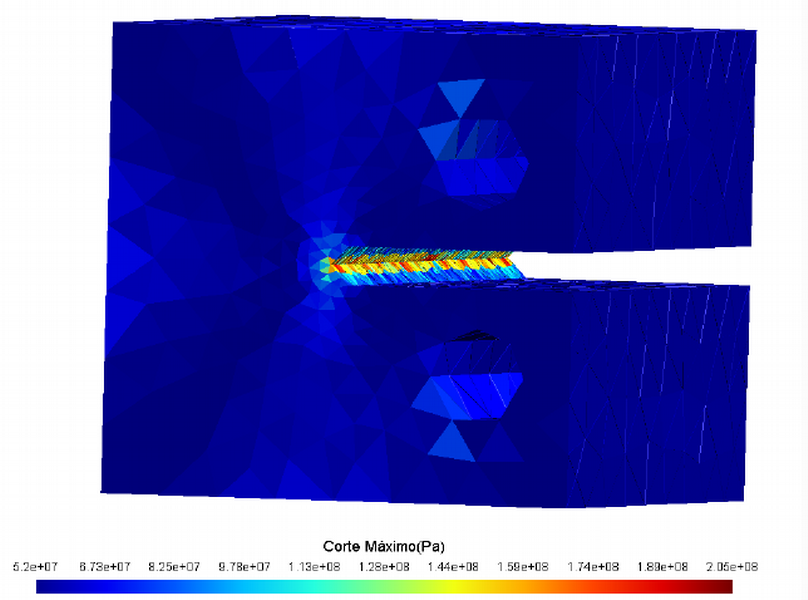
\includegraphics[height=0.5\textheight,width=\textwidth]{/home/mariano/CuadernoTrabajo/CV/SLI/03-Teaching/02.png}
\vspace{0.5cm}
\begingroup
\small
We guide students make while they build their own 
implementation of the Finite Element Method 
in any language they choose.
\endgroup
\vspace{0.5cm}

\end{center}
\end{columns}

\end{frame}
